\chapter{Easy burning subproblems}\label{chapter:where-easy}

Not much work has been done which gave algorithms for easy (polynomial time) burning of graph classes. This chapter includes the findings which show that optimal burning can be performed on certain graph classes in polynomial time.

\section{Burning path or cycle (already discussed)}

We have already discussed in \Cref{section:burn-path} that a simple path or cycle can be burned optimally in polynomial time.

\section{Burning split graphs}

\subsection{Burning connected split graphs}

If the clique $C$ and the independent set $I$ are given for an arbitrary split graph (see \Cref{subsection:split-graphs}) $G$, then we can burn a connected split graph in two or three steps \cite{Kare2019}. \Cref{algorithm:burn-connected-split-graphs} shows how to burn a connected split graph optimally in polynomial time.

\begin{algorithm}\label{algorithm:burn-connected-split-graphs}
Given the input $(G,\ C,\ I)$, where $G$ is the input connected split graph, $C$ (represents the clique) and $I$ (represents the the independent set), both are subsets of $G.V$, perform the following steps.
\end{algorithm}

\textbf{\textit{Step 1.}} Time step $t=0$.\\
$B$ stores the set of vertices which are burned, initially $B=\phi$. $S$ will store an optimal burning sequence of $G$, initially $S=\phi$.

\textbf{\textit{Stage 2.}} Time step $t=1$.\\
$S=\{c\}$ where $c$ is an arbitrary vertex in $C$, preferably adjacent to at least one vertex in $I$. $B=\{c\}$. If $B=G.V$, then return $S$.

\textbf{\textit{Stage 3.}} Time step $t=2$.\\
$S = S\cup \{i\}$, where $i$ is an arbitrary unburned vertex in $I$ (preferably, such that $i$ is not connected to the same vertex in $C$ as $S[|S|]$) or $C$. $B = B \cup \{i\} \cup G.Adj[B]$.\\
If $B=G$, then return $S$.

\textbf{\textit{Stage 4.}} Time step $t=3$.\\
$S = S\cup \{i\}$, where $i$ is an arbitrary unburned vertex in $I$. $B = B \cup \{i\} \cup G.Adj[B]$.\\
Return $S$.\\

\Cref{algorithm:burn-connected-split-graphs} runs in linear time, given that $C$ and $I$ are computed already. For a connected split graph $G$, the burning number $b(G)$ is $2$ or $3$. It is interesting to observe that even if the split graph is not a connected graph, then also we can burn the graph in polynomial time $O(n)$, given that the first fire source is placed in $C$.

\subsection{Burning general split graphs}

\begin{theorem}\label{theorem:burning-general-split-graphs}
    For an arbitrary split graph $G$, the first fire source in an optimal burning sequence should be placed on $c$, an arbitrary vertex in $C$ (representing the clique), a subgraph of $G.V$.
\end{theorem}

\begin{proof}
\noindent \textbf{General construction}: Let $G$ be a split graph of $n$ vertices such that $C = \{c_1, c_2, c_3, . . ., c_{n-1}\}$ is a complete subgraph of $G$ of size $n-1$, and $I = \{i\}$ is the independent set excerpt of $G$. $i$ is not connected to any vertex in $G$. Let the optimal burning sequence be $S^\prime = (y_1, y_2, y_3, . . ., y_{k^\prime})$ be of $k^\prime$ vertices. Consider for contradiction that the fire source $y_1$ is placed on $i$, and yet we are able to burn $G$ in the mininimum possible time steps.\\

\noindent \textbf{Example construction and solution}: Let $n=4$. When $y_1$ is placed on $i$, a burning sequence required to burn $G$ is $(i, c_1, c_2)$. This is shown in figure \thech.2.

\begin{figure}
    \centering
    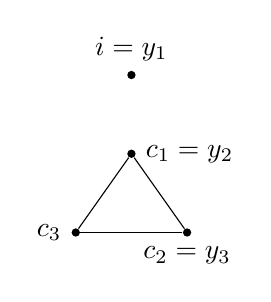
\begin{tikzpicture}
        \node [circle, fill=black, inner sep=0pt, minimum size=3pt, label=right:{$c_1 = y_2$}] (A) at (0,0) {};
        \node [circle, fill=black, inner sep=0pt, minimum size=3pt, label=below:{$c_2 = y_3$}] (B) at (.707,-1) {};
        \node [circle, fill=black, inner sep=0pt, minimum size=3pt, label=left:{$c_3$}] (C) at (-.707,-1) {};
        
        \node [circle, fill=black, inner sep=0pt, minimum size=3pt, label=above:{$i = y_1$}] (D) at (0,1) {};
        
        \draw (A) -- (B); \draw (A) -- (C); \draw (B) -- (C);
        %\draw (A) -- (D); \draw (B) -- (E); \draw (C) -- (F);
    \end{tikzpicture}
    \caption{If the first fire source is placed on $i$, then the burning sequence is $i,c_1,c_2$. If, otherwise, the first fire source is placed on $c_1$ (for example), then the burning sequence is $c_1,i$}
    \label{figure:burning-general-split-graphs}
\end{figure}

On the other hand, if $y_1$ were placed on $c_1$, an arbitrary vertex in $C$, a burning sequence required to burn $G$ is $(c_1, i)$.
\end{proof}

Given that the vertices of $I$ are connected to atmost one vertex in $C$, then in an optimal burning sequence, we can put the first fire source on a vertex in $I$ iff there are atmost $2$ vertices in $I$ which are disconnected from $C$. 
If otherwise the vertices of $I$ are connected to more than one vertices of $C$, then in an optimal burning sequence, we can put the first fire source on a vertex in $I$ iff there are atmost $3$ vertices in $I$ which are disconnected from $C$.

\Cref{theorem:burning-general-split-graphs} lays the foundation of algorithm \Cref{algorithm:burning-general-split-graphs}, which computes an optimal burning sequence for disconnected split graphs in $O(n)$.

\begin{algorithm}\label{algorithm:burning-general-split-graphs}
    Given the input $(G,\ C,\ I)$, where $G$ is a connected split graph, $C$ represents the clique, $C\subseteq G.V$, and $I$ represents the independent set in $G$, $I\subseteq G.V$, perform the following steps.
\end{algorithm}

\textbf{\textit{Step 1.}} Time step $t=0$.\\
$B$ stores the set of vertices which are burned, initially $B=\phi$. $S$ will store an optimal burning sequence of $G$, initially $S=\phi$.

\textbf{\textit{Stage 2.}} Time step $t=1$.\\
$S=\{c\}$ where $c$ is an arbitrary vertex in $C$, preferably adjacent to at least one vertex in $I$. $B=\{c\}$. If $B=G.V$, then return $S$.

\textbf{\textit{Stage 3.}} Time step $t=2$.\\
$S = S\cup \{i\}$, where $i$ is an arbitrary unburned vertex in $I$ (preferably, such that $i$ is not connected to the same vertex in $C$ as $S[|S|]$) or $C$. $B = B \cup \{i\} \cup G.Adj[B]$.\\
If $B=G$, then return $S$.

\textbf{\textit{Stage 4.}} Perform the following steps until $B=G$.

\textbf{\textit{Stage 4.1.}} Time step $t=t+1$.\\
$S = S\cup \{i\}$, where $i$ is an arbitrary unburned vertex in $I$. $B = B \cup \{i\} \cup G.Adj[B]$.\\

\textbf{\textit{Stage 5.}} Return $S$.

\section{Burning cographs}

Refer to the definition of \textit{cographs} in \Cref{subsection:cographs}. In a cograph $G$, each vertex in $G$ is atmost at a distance $2$ or $3$ from $v$, an arbitrary vertex in $G$ \cite{Kare2019}. Hence we can burn a cograph in atmost $3$ steps.

% \bibliography{ref.bib}
% \bibliographystyle{plain}